% Chapter 1

\chapter{Introducción general}

\label{Chapter1}
\label{IntroGeneral}

En este capítulo se introduce el dominio de la telemetría embebida aplicada a motocicletas. Se presentan el contexto, la motivación, el estado del arte y los objetivos del trabajo.

%----------------------------------------------------------------------------------------

% Define some commands to keep the formatting separated from the content
\newcommand{\keyword}[1]{\textbf{#1}}
\newcommand{\tabhead}[1]{\textbf{#1}}
\newcommand{\grados}{$^{\circ}$}

%----------------------------------------------------------------------------------------
\section{Introducción a la telemetría embebida en motocicletas}
\label{sec:intro-general-tema}

Existe una amplia variedad de sistemas embebidos en la actualidad. Se encuentran en lo cotidiano en electrodomésticos, equipos médicos, instrumentación industrial, sistemas de transporte, entre muchos otros. En todos los casos, un firmware dedicado ejecuta la lógica que define la funcionalidad del producto y condiciona su confiabilidad en el tiempo.

Un sistema embebido es un sistema computacional orientado a una función acotada, integrado en un producto mayor y sujeto a límites de tamaño, consumo, costo y tiempo de respuesta. A diferencia de un equipo de uso general, el hardware y el software se conciben de forma conjunta para adquirir señales, controlar un proceso o registrar información en tiempo acotado.

En el ámbito vehicular, los sistemas embebidos abordan distintos dominios de aplicación. Uno de ellos es la telemetría vehicular, que concentra la adquisición, sincronización, almacenamiento, y transmisión de magnitudes cinemáticas y físicas. En la figura~\ref{fig:telemetria-vehicular-conceptual} se representa de forma esquemática la cadena típica en la que intervienen el vehículo, un dispositivo embebido que adquiere y registra datos, y una etapa de visualización de la información para el usuario. En competición y en flotas profesionales, este tipo de soluciones están ampliamente extendidas. En el uso particular del conductor, la demanda se orienta hacia equipos compactos, confiables, y de costo moderado \citep{garcia2026_moto_telemetry}.

\begin{figure}[htbp]
	\centering
	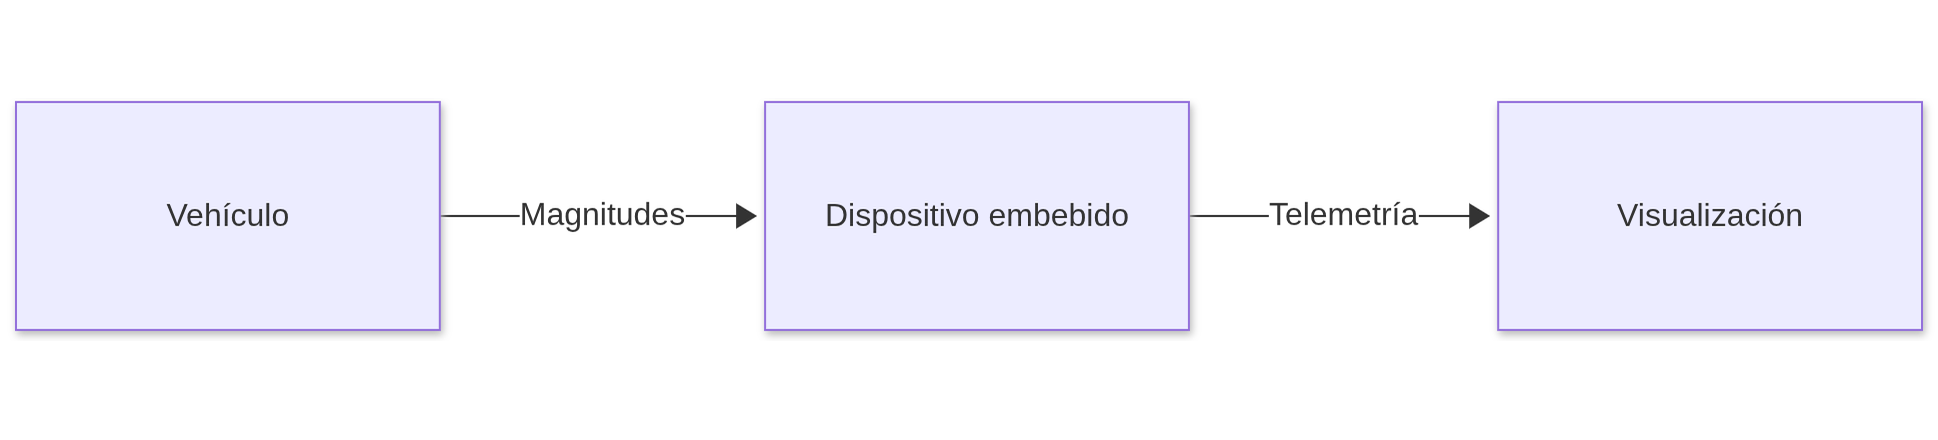
\includegraphics[width=0.92\textwidth]{Figures/telemetria-vehicular-conceptual.png}
	\caption{Vista conceptual de un sistema de telemetría vehicular.}
	\label{fig:telemetria-vehicular-conceptual}
\end{figure}

%----------------------------------------------------------------------------------------
\section{Contexto y motivación}
\label{sec:contexto-motivacion}

La conducción en motocicleta impone condiciones dinámicas exigentes. El usuario enfrenta cambios rápidos de velocidad, inclinación en curvas y mayor exposición a maniobras bruscas o a incidentes. Un dispositivo embebido montado en la motocicleta puede servir a la vez como instrumento de medición y como un respaldo de datos de conducción, con un rol análogo al de una caja negra en otros medios de transporte.

El proceso que se busca instrumentar es ese entorno de conducción. Se requiere registrar variables cinemáticas y geográficas, identificar maniobras bruscas o situaciones de riesgo y conservar un historial utilizable después del recorrido o ante un incidente. Muchos conductores recurren a aplicaciones en el teléfono móvil. Esas aplicaciones no están integradas al vehículo, dependen de sensores del teléfono y no garantizan registro autónomo en él. Los dispositivos profesionales ofrecen alta confiabilidad, pero exigen instalación, configuración y mantenimiento más complejos, además de costos elevados y ecosistemas cerrados poco accesibles para un uso particular.

Las restricciones de tamaño, consumo y costo se combinan con condiciones físicas exigentes en el vehículo, como vibración, variación térmica y espacio limitado para el montaje. Esas limitaciones obligan a una arquitectura optimizada. El microcontrolador debe coordinar periféricos en paralelo, sostener tasas de muestreo adecuadas y ejecutar lógica de análisis en tiempo acotado sin depender de servicios remotos permanentes. La plataforma debe reunir adquisición multivariable, persistencia local y enlace de corto alcance hacia una aplicación móvil en el teléfono.

La motivación del trabajo es cubrir esa brecha con un sistema embebido dedicado. Se prioriza la medición orientada al vehículo, el almacenamiento en tarjeta de memoria removible y el enlace inalámbrico sin conectividad celular en el dispositivo. El prototipo integra un microcontrolador STM32 (STMicroelectronics) sobre la placa de desarrollo NUCLEO-F446RE, sensado inercial, receptor de posicionamiento global, registro en tarjeta microSD y comunicación por Bluetooth de baja energía (BLE) con la aplicación móvil.

%----------------------------------------------------------------------------------------
\section{Estado del arte}
\label{sec:estado-arte}

Durante el relevamiento sobre telemetría embebida en motocicletas se constató que el mercado profesional está dominado por plataformas cerradas, probadas en competición y en desarrollo de producto \citep{garcia2026_moto_telemetry}. Fabricantes como AiM Technologies, MoTeC y 2D Datarecording ofrecen dispositivos con unidad de medición inercial integrada, posicionamiento global, interfaces de bus de área de controlador (CAN), y software propietario de análisis \citep{aim_evo5,aim_mxl2,motec_c187,data2d_moto}. Esas soluciones alcanzan alta confiabilidad, pero suelen implicar costos elevados, formatos de datos poco abiertos y poca extensibilidad para algoritmos propios de análisis de conducción.

En la tabla~\ref{tab:comercial-telemetria} se resume un conjunto de las alternativas comerciales de nivel profesional relevadas.

\begin{table}[htbp]
	\centering
	\caption{Alternativas comerciales representativas de telemetría para vehículos y motocicletas.}
	\label{tab:comercial-telemetria}
	\begin{tabular}{|p{2.2cm}|p{2.4cm}|p{4.2cm}|p{4.5cm}|}
		\hline
		\tabhead{Producto} & \tabhead{Fabricante} & \tabhead{Capacidades principales} & \tabhead{Limitaciones} \\
		\hline
		EVO5 & AiM Technologies \citep{aim_evo5} & Canales configurables, posicionamiento global, bus CAN, y software Race Studio & Arquitectura cerrada. Costo elevado en configuraciones completas \\
		\hline
		MXL2 & AiM Technologies \citep{aim_mxl2} & Acelerómetro y giroscopio internos, posicionamiento global, entradas analógicas, y memoria interna & Mismo ecosistema propietario \\
		\hline
		C187 & MoTeC \citep{motec_c187} & Display a color, registro de datos, posicionamiento global, y software MoTeC i2 & Enfoque competición. Hardware y licencias de alto costo \\
		\hline
		Sticklogger V2/V3/V4 & 2D Datarecording \citep{data2d_moto} & Registro en memoria USB 3.0, señales CAN, analógicas, y digitales, y configuración vía USB & Plataforma cerrada. Enfoque competición y entornos exigentes \\
		\hline
	\end{tabular}
\end{table}

En el ámbito académico, las publicaciones abordan registradores de eventos, reconstrucción de trayectorias, detección de colisiones, y plataformas embebidas de bajo costo. En Gelmini y col., se propuso un algoritmo de detección y clasificación de colisiones para vehículos de dos ruedas a partir de mediciones inerciales y de posicionamiento global \citep{gelmini2021_crash}. En Smaiah y col., se reconstruyeron trayectorias de motocicleta con un sistema multisenorial de bajo costo \citep{smaiah2018_trajectory}. En García Cuadra y col., se publicó una plataforma embebida abierta sobre microcontrolador STM32H7, con posicionamiento global de alta precisión, unidad de medición inercial, bus CAN con extensión CAN-FD, y enlace celular \citep{garcia2026_moto_telemetry}. Ese aporte evidencia la viabilidad de arquitecturas abiertas frente a registradores cerrados de competición.

%----------------------------------------------------------------------------------------
\section{Objetivos del trabajo}
\label{sec:objetivos}

Esta sección presenta los objetivos del trabajo y el alcance del prototipo desarrollado. Primero se define el objetivo general, seguido de los objetivos específicos. Finalmente, se establece el alcance del proyecto, detallando qué aspectos fueron implementados y cuáles quedaron excluidos.

\subsection{Objetivo general}
\label{sec:objetivo-general}

El objetivo general del trabajo fue diseñar e implementar un sistema embebido de telemetría y detección de eventos para motocicletas, capaz de adquirir variables cinemáticas y geográficas, registrar datos de forma local y comunicarse con una aplicación móvil en el teléfono.

\subsection{Objetivos específicos}
\label{sec:objetivos-especificos}

Los objetivos específicos fueron los siguientes:

\begin{enumerate}
	\item Seleccionar e integrar una plataforma de hardware basada en la familia de microcontroladores STM32 y los módulos de sensado necesarios para posicionamiento global y medición inercial.
	\item Desarrollar el firmware que permita adquirir, sincronizar y registrar muestras de sensores con tasas adecuadas para el análisis de la conducción.
	\item Implementar almacenamiento persistente en una tarjeta de memoria removible, con formatos de registro que permitan un análisis posterior.
	\item Establecer comunicación BLE con la aplicación móvil para la transferencia de telemetría.
	\item Incorporar lógica para identificar maniobras de conducción relevantes a partir de las señales adquiridas, como base para puntuación y alertas.
	\item Verificar el funcionamiento del sistema mediante ensayos sobre el hardware, el firmware, y la integración con la aplicación móvil.
\end{enumerate}

\subsection{Alcance}
\label{sec:alcance}

El alcance comprendió el diseño e implementación de un prototipo embarcado sobre la placa NUCLEO-F446RE, el firmware asociado y la aplicación móvil para el envío de telemetría por BLE. Se priorizó la adquisición multivariable, la persistencia local y la interfaz con el usuario móvil.

En el firmware se incluyó un sistema operativo de tiempo real para ejecutar de forma concurrente el muestreo de sensores, el registro en tarjeta de memoria removible y el enlace BLE. Esa organización buscó aislar las rutinas periódicas de las operaciones de entrada-salida de mayor latencia y mantener acotados los tiempos de respuesta del dispositivo.

\begin{figure}[htbp]
	\centering
	\includegraphics[width=0.9\textwidth]{"Figures/Diagrama bloques.png"}
	\caption{Diagrama de bloques del dispositivo.}
	\label{fig:alcance-diagrama-bloques}
\end{figure}

Quedaron fuera del alcance cualquier tipo de certificación u homologación del dispositivo, la conexión con la electrónica de la motocicleta mediante bus CAN u otros enlaces de diagnóstico, y el uso de servicios en la nube para almacenamiento remoto. Tampoco se buscó igualar el desempeño ni el costo de dispositivos comerciales de competición. El foco fue proveer una solución extensible y de costo moderado para conductores particulares.
